We describe multiple equivalent constructions of a toric variety starting from the data
of a polytope $P$ subject to certain conditions. Each of 
the constructions will yield us a space $X_i(P)$ which will all be 
equivariantly diffeomorphic to each other as smooth manifolds. 


% Depending on the nature of the construction, $X_i(P)$ will either be 
% a projective toric variety or a toric symplectic manifold, and these 
% two classes of spaces can be identified with each other via the image 
% of their moment maps.



\subsection{Delzant polytopes}
Let $V$ be a real vector space of dimension $n$ and let $V_\Z$
be a lattice inside $V$. Given 
$N$ linear functionals $a_i \in V^*$ preserving $V_\Z$ and $N$ integers $\lambda_i$
the set \begin{align*}
P = \{ v \in V \mid a_i(v) + \lambda_i \geq 0 \text{ for all } i \}.
\end{align*} is called a \emph{rational polyhedron}. It is called 
a \emph{rational polytope} if it is bounded. We will assume that $P$ is a
rational polytope throughout this paper. A polytope $P$ has \emph{facets} \begin{align*}
F_i = \{ v \in P \mid a_i(v) + \lambda_i = 0 \}
\end{align*} and \emph{faces} which are intersections of facets. 
The \emph{vertices} of $P$ are the 0-dimensional faces of $P$ and 
the \emph{edges} of $P$ are the 1-dimensional faces of $P$.
We say $P$ is: \begin{itemize}
    \item \emph{simple} if exactly $n$ edges meet at each vertex
    \item \emph{smooth} if the edges meeting at each vertex form a basis for $V_\Z$
    \item \emph{Delzant} if $P$ is simple and smooth
\end{itemize}

\begin{example}
    The right triangle $P = \{ (x,y) \in \R^2 \mid x \geq 0, y \geq 0, x + y \leq 1 \}$ is a 
    Delzant polytope. The standard tetrahedron $P\subset\R^3$ is not Delzant because the
    top vertex is not simple.
\end{example}
We begin by stating the correspondence we are interested in.
\begin{theorem}\label{thm:delzant}
    [Delzant] There is a correspondence between Delzant polytopes up to $\GL(n,\Z)$ 
    and translation, and toric symplectic manifolds up to equivariant symplectomorphism.
\end{theorem}

\begin{theorem}
    There is a correspondence between Delzant polytopes up to $\GL(n,\Z)$
    and translation, and smooth projective toric varieties with a particular choice
    of very ample line bundle, up to equivariant isomorphism.
\end{theorem}

\subsection{Moment maps}
Let $(M,\omega)$ be a symplectic manifold. The nondegeneracy of $\omega$ allows us to
pair vector fields with 1-forms. We say that a vector field $X$ is \emph{Hamiltonian} if
the corresponding 1-form $\iota_X\omega = \omega(X,\cdot)$ is exact, in which case 
it is equal to $dH$ for some smooth function $H$. The function $H$ is called a
\emph{Hamiltonian} of $X$. 

\hfill

Given a Lie group $G$ acting on $M$ by symplectomorphisms,
the Lie algebra $\mathfrak{g}$ acts on $M$ by symplectic vector fields.
This linearized action of $\mf g$ is given by the expression
\begin{align*}
    X_\zeta(m) = \frac{d}{dt}\Big|_{t=0} \exp(t\zeta)\cdot m
\end{align*} where we interpret the given expression via parallel transport along the flow of $\zeta$.

\begin{remark}
    In general, whenever we have a Lie group $G$ acting on a manifold $M$, we get a linearized
    action of $\mf g$ on $\Gamma(E)$ for any vector bundle $E$ over $M$. For the trivial 
    line bundle $E = M\times \R$ we have $\Gamma(E) = C^\infty(M)$ and the linearized action
    of $\mf g$ on $C^\infty(M)$ is given by the Lie derivative of 
    the function along the vector field.
\end{remark}

\begin{example}
    Consider $G = \SL(2,\C)$ acting on $\P^1$ by linear fractional transformations. Explicitly
    we have \begin{align*}
        \begin{pmatrix}
            a & b \\
            c & d
        \end{pmatrix} \cdot [z_0:z_1] = [az_0 + bz_1 : cz_0 + dz_1]
    \end{align*} The Lie algebra $\mf{sl}(2,\C)$ is generated by the matrices \begin{align*}
        E = \begin{pmatrix}
            0 & 1 \\
            0 & 0
        \end{pmatrix} \quad F = \begin{pmatrix}
            0 & 0 \\
            1 & 0
        \end{pmatrix} \quad H = \begin{pmatrix}
            1 & 0 \\
            0 & -1
        \end{pmatrix}
    \end{align*} Writing down the exponential, we find that \begin{align*}
        \exp(tE) = I + tE \quad \text{since } E^2 = 0
        \implies \exp(tE)\cdot [z_0:z_1] = [z_0 + tz_1 : z_1]
    \end{align*} On an affine chart, the action of $E$ is given by $z \mapsto z + t$ and
    we compute \begin{align*}
        \frac{d}{dt}\Big|_{t=0} z + t = 1 \implies X_E(z) = \frac{\partial}{\partial z}
    \end{align*} Similarly we compute \begin{align*}
        \exp(tH) = \begin{pmatrix}
            e^t & 0 \\
            0 & e^{-t}
        \end{pmatrix} \implies \exp(tH)\cdot [z_0:z_1] = [e^tz_0 : e^{-t}z_1]
    \end{align*} which looks like $z\mapsto e^{2t}z$ on an affine chart, which gives us
     \begin{align*}
        \frac{d}{dt}\Big|_{t=0} e^{2t}z = 2z \implies X_H(z) = 2z \frac{\partial}{\partial z}
    \end{align*} Finally we compute \begin{align*}
        \exp(tF) = 1 + tF \implies \exp(tF)\cdot [z_0:z_1] = [z_0 : z_1 + tz_0]
    \end{align*} On an affine chart this transformation looks like $z\mapsto z/(1+tz)$
    and we compute \begin{align*}
        \frac{d}{dt}\Big|_{t=0} \frac{z}{1+tz} = -z^2 \implies X_F(z) = -z^2\frac{\partial}{\partial z}
    \end{align*} In particular we get a map $\mf{sl}(2,\C) \to \Gamma(T\P^1)$ given by
    \begin{align*}
        E &\mapsto \frac{\partial}{\partial z} \\
        H &\mapsto 2z\frac{\partial}{\partial z} \\
        F &\mapsto -z^2\frac{\partial}{\partial z}
    \end{align*} which is the standard action of $\mf{sl}(2,\C)$ on $T\P^1$. This map in fact 
    extends to an isomorphism between the enveloping algebra $U(\mf{sl}(2,\C))$ and 
    the algebra of differential operators on $\cD_{\text{hol}}(\P^1)$. This is a 
    shadow of the Beilinson-Bernstein localization theorem (cf. \cite{htt}).
\end{example}

We say that the
action of $G$ is \emph{weakly Hamiltonian} 
if for every $\zeta\in\mf g$ the corresponding vector field $X_\zeta$ is Hamiltonian,
i.e. $\iota_{X_\zeta}\omega = dH_\zeta$ for some smooth function $H_\zeta$. The $H_\zeta$
is determined only up to a constant, so choose the map $\mf g \to C^\infty(M)$ given by 
$\zeta \mapsto H_\zeta$ to be linear. If the map can be chosen to be equivariant with respect
to the adjoint action of $G$ on $\mf g$, then the action of $G$ is called \emph{Hamiltonian}.
In this case, there is a map $\mu : M \to \mf g^*$ called the \emph{moment map} defined by
\begin{align*}
    H_\zeta(m) := \langle \mu(m), \zeta \rangle
\end{align*}
If the action of $G$ is Hamiltonian, then the moment map is $G$-equivariant and unique up 
to the addition of a constant. When $G = T$ is a torus, the adjoint action 
is trivial and the moment map $\mu : M \to \mf t^*$
is $T$-invariant.

\begin{theorem}\label{thm:ags}
    [Atiyah-Guillemin-Sternberg Convexity Theorem] Let $M$ be a compact connected symplectic manifold with a
    Hamiltonian $T$-action. Then the image of the moment map is a convex polytope 
    in $\mf t^*$ whose vertices are the image of the fixed points of the $T$-action.
\end{theorem}
\begin{proof}
    See \cite{mcduff-salamon}.
\end{proof}

We say $M$ is a \emph{toric symplectic manifold} in the sense of Theorem \ref{thm:delzant}
if $(M,\omega)$ is a compact connected symplectic manifold
with a effective (meaning no element of $T$ acts trivially) Hamiltonian $T$-action.

\begin{proposition}
    Let $M\subset \C\P^n$ be a smooth projective toric variety embedded by a line bundle.
    Then $M$ is equivariantly symplectomorphic to a toric symplectic manifold.
\end{proposition}
\begin{proof}
$\C\P^n$ carries a natural symplectic form $\omega$ 
called the Fubini-Study form. Any smooth projective toric variety $M$ embedded
in projective space carries a symplectic form $\omega$ induced by pulling 
back the Fubini-Study form. Moreover, the action of $T$ on $M$
 is Hamiltonian with respect to $\omega$.
\end{proof}

\hfill

Conversely, given a toric symplectic manifold $(M,\omega)$, we can associate a 
smooth projective toric variety to the moment polytope $\mu(M)$ which will be
equivariantly symplectomorphic to $M$.

\subsection{Symplectic reduction}
We describe how to construct $M$ as the symplectic reduction of affine space $\C^N$ for 
a particular moment map. In particular, $M$ carries a natural symplectic form $\omega$ and 
a Hamiltonian $T$-action.
This section follows \cite{lsg}. 

\hfill 

Let $P$ be a Delzant polytope.
There are maps \begin{align*}
    \pi:\R^N&\to\R^n\\
    e_i &\mapsto a_i
\end{align*} and the induced map \begin{align*}
    \pi: \R^N/\Z^N\to\R^n/\Z^n 
\end{align*} of tori, which give rise to the following short exact sequences. \begin{align}\label{eq:ses1}
    1\to K \to \T^N \to \T^n \to 1
\end{align} \begin{align*}
    0\to k \to \R^N\to \R^n\to 0
\end{align*} The dual of the second sequence gives \begin{align*}
    0 \to (\R^n)^* \to (\R^N)^* \to k^* \to 0
\end{align*} and denote the map $i^* : (\R^N)^*\to k^*$. Now consider $\C^N$
with the standard symplectic form $\omega = \sum dz_i\wedge d\bar z_i$ and the 
standard Hamiltonian torus action \begin{align*}
    (e^{i\theta_1},\dots,e^{i\theta_N})\cdot(z_1,\dots,z_N) = (e^{i\theta_1}z_1,\dots,e^{i\theta_N}z_N)
\end{align*} and corresponding moment map \begin{align*}
    \phi:\C^N&\to(\R^N)^* \\
    \phi(z_1,\dots,z_N) &= -\pi(|z_1|^2,\dots,|z_N|^2) + (\lambda_1,\dots,\lambda_N)
\end{align*}
The subtorus $K$ acts on $\C^N$ via restriction and the restricted action is 
Hamiltonian. Moreover, the moment map for the action of $K$ is given by $i^*\circ\phi:M\to k^*$.

\hfill

Let $Z = (i*^\circ \phi)^{-1}(0)$ be the zero level set of the moment map. The following 
claims are all justified in \cite{lsg}.

\begin{lemma}
    $Z$ is compact and $K$ freely acts on $Z$. 
\end{lemma}

The following theorem tells us that the orbit space $Z/K$ is a symplectic manifold.

\begin{theorem}{\label{thm:reduction}}
    [Marsden-Weinstein-Meyer] Let $G$ be a compact group and let $(M,\omega)$ be a symplectic manifold with a
    Hamiltonian $G$-action. Let $i:\mu^{-1}(0)\to M$ be the inclusion of the zero level set of the moment map.
    Assume $G$ acts freely on $\mu^{-1}(0)$. Then \begin{itemize}
        \item the orbit space $M_{\text{red}} = \mu^{-1}(0)/G$ is a smooth manifold
        \item $\pi:\mu^{-1}(0)\to M_{\text{red}}$ is a principal $G$-bundle
        \item there is a unique symplectic form $\omega_{\text{red}}$ on $M_{\text{red}}$ such that $\pi^*\omega_{\text{red}} = i^*\omega$
    \end{itemize}
\end{theorem}
Symplectic reduction realizes one direction of Delzant's correspondence.
\begin{proposition}
    The reduced space $X_1(P) := Z/K$ is a toric symplectic manifold with moment map image $P$.
\end{proposition}

\subsection{Monoid algebra}
Let $P$ be a Delzant polytope. Consider the cone \begin{align*}
    \sigma_P = \{ (v,t) \in V \times \R \mid v \in tP, t \geq 0 \}
\end{align*} The lattice points of this cone 
form a semigroup $S_P$. Define the space \begin{align*}
    X_2(P) = \Proj \C[S_P]
\end{align*} 

\begin{proposition}
    The space $X_2(P)$ is a smooth projective toric variety.
\end{proposition}
This follows from general theory of projective toric varieties. We 
refer the reader to chapter 2 of \cite{cls} for a detailed exposition.

\subsection{Projective GIT}
Let $P$ be a Delzant polytope. Complexifying (\ref{eq:ses1}), we get \begin{align*}
    1\to K_\C \to T_\C^N \to T_\C^n \to 1 
\end{align*} Let $F_i$ denote the facets of $\Delta$ and for any $z = (z_1,\dots,z_N)\in\C^n$ let $F_z := \cap_{z_i = 0}F_i$.
Consider the set \begin{align*}
    U = \{z\in\C^n: F_z \neq \emptyset\}
\end{align*} Then the quotient $X_3(P) = U/K_\C$ is a manifold with an action of $T_\C^N/K_\C = T_\C^n$. It 
is a smooth projective toric variety \red{because it is a projective GIT quotient}.

\begin{remark}
    There is a surjective map from $X^{ss}$ to $X//G$. Two points in $X^{ss}$ lie in the same fiber of this map if and only if the closures of their 
    $G$-orbits intersect. In this case, the $K_\C$ orbits are closed. See \cite{proudfoot} for more details.
\end{remark}
\subsection{Kempf-Ness theorem}
We want to compare the symplectic quotient to the projective GIT quotient.  First recall
that if $K$ is a real compact group, then its complexification $G := K_\C$ is a 
complex Lie group which contains $K$ and $\mf g = \mf k \oplus i\mf k$ is the complexification
 of $\mf k$. See \cite{hoskins} for more details about the following theorems.

\begin{theorem}
    Complexification defines a bijection between the isomorphism
    classes of compact real Lie groups and complex reductive groups.
\end{theorem}
The following theorem of Kempf-Ness states a relationship between the symplectic quotient and the GIT quotient.
\begin{theorem}{\label{thm:kempf-ness}}
    [Kempf-Ness] 
    Let $G$ be a complex reductive group acting on a smooth complex projective variety 
    $X\subset \P^n$. Let $K$ be a maximal compact subgroup of $G$ and suppose $K$ 
    is connected and acts on $X$ Hamiltonianly. Let $\mu:X\to\mf k^*$ be the moment map. 
    Then the inclusion $\mu^{-1}(0)\to X$ induces a homeomorphism \begin{align*}
        \mu^{-1}(0)/K \to X//G
    \end{align*}
\end{theorem}

\begin{remark}
    \red{We should say more about this theorem}
\end{remark}

\subsection{Fans and abstract toric varieties}

Let \( T \) be an \( n \)-dimensional torus with character group \( M \),
 and let \( N = \operatorname{Hom}_{\mathbb{Z}}(M, \mathbb{Z}) \) be
  the dual lattice, with pairing denoted \( \langle , \rangle \). Recall that Theorem \ref{thm:delzant} gives a correspondence between Delzant polytopes 
and smooth projective toric varieties equipped with a very ample line bundle.
Forgetting the embedding, we pass to the abstract toric variety, whose combinatorics 
ends up being encoded in the data of a fan.

\begin{definition}
    A \emph{fan} $\Sigma$ in a real vector space $N$ is a collection of cones
    $\sigma$ such that \begin{itemize}
        \item $\sigma$ is a strongly convex polyhedral cone
        \item if $\sigma\in\Sigma$ and $\tau$ is a face of $\sigma$, then $\tau\in\Sigma$
        \item the intersection of any two cones in $\Sigma$ is a face of each
    \end{itemize}
\end{definition}

Given a Delzant polytope $P$, there is a fan $\Sigma_P$ in $N_\R$ obtained by taking 
normal directions to the facets of $P$. The fan $\Sigma_P$ is called the \emph{normal fan} of $P$
and it is a combinatorial object which encodes an equivariant atlas of charts for the toric variety $X(P)$.

\begin{definition}
    A fan $\Sigma$ is \emph{complete} if the union of the cones in $\Sigma$ is all of $N_\R$.
    A fan $\Sigma$ is \emph{nonsingular} if for each $k$-dimensional cone $\sigma\in\Sigma$,
    there exist $k$ lattice vectors $v_1,\dots,v_k$ such that $\{v_1,\dots,v_k\}$ generate $\sigma$
    and $v_1,\dots,v_k$ can be extended to a basis of $N$.
    A fan $\Sigma$ is \emph{projective} if there is a rational polytope $P$ such that $\Sigma$ is the normal fan of $P$.
\end{definition}

As the geometric language suggests, the toric variety $X(\Sigma)$ 
corresponding to a fan $\Sigma$ is complete if and only if the fan is complete,
and $X(\Sigma)$ is smooth if and only if the fan is nonsingular.

See \cite{cls} for more details. 



\begin{example}
    Consider the unit right triangle with corresponding normal fan
    \begin{center}
        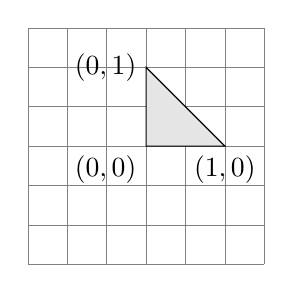
\begin{tikzpicture}[scale=0.5]
            \draw[step=1cm,gray,very thin] (-3,-3) grid (3,3);
            \filldraw[fill=gray!20, draw=black] (0,0) -- (2,0) -- (0,2) -- cycle;
            \node at (0,0) [below left] {$(0,0)$};
            \node at (2,0) [below] {$(1,0)$};
            \node at (0,2) [left] {$(0,1)$};
        \end{tikzpicture}
        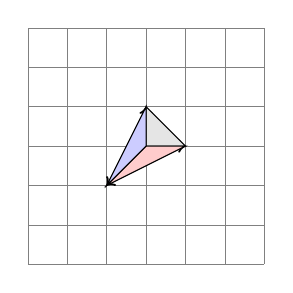
\begin{tikzpicture}[scale=0.5]
            \draw[step=1cm,gray,very thin] (-3,-3) grid (3,3);
            \draw[thick,->] (0,0) -- (1,0);
            \draw[thick,->] (0,0) -- (0,1);
            \draw[thick,->] (0,0) -- (-1,-1);
            % fill in the upper right quadrant
            \filldraw[fill=gray!20, draw=black] (0,0) -- (1,0) -- (0,1) -- cycle;
            % fill in the region from pi/2 to 5pi/4 
            \filldraw[fill=red!20, draw=black] (0,0) -- (-1,-1) -- (1,0) -- cycle;
            % fill in the region from 5pi/4 to 3pi/2
            \filldraw[fill=blue!20, draw=black] (0,0) -- (-1,-1) -- (0,1) -- cycle;
        \end{tikzpicture}
    \end{center} 
    Note that the fan has three 2-dimensional cones which are filled in.
    These cones represent the three standard coordinate charts of $\P^2$ given by
    $x_i \neq 0$ for $i = 0,1,2$. The isosceles right triangle with
    side lenghth $a$ corresponds to the $a$-th Veronese 
    embedding of $\P^2$.
\end{example}
Fans are more friendly objects for algebraic geometers and 
one can read further about them in \cite{cls}. The data of a fan,
and in particular the primitive edge vectors (defined as the generators of the rays of the fan),
will prove important in our discussion on equivariant cohomology.

\subsection{Prequantization}
Manifolds equipped with integral symplectic forms admit prequantization line bundles.
In particular we have the following theorem. 

\begin{theorem}
    Let $(M,\omega)$ be a symplectic manifold. Suppose that $[\omega]$ is integral. Then 
    there exists a "prequantization" line bundle $\cL \to M$ with $c_1(\cL) = [\omega]$ and a Hermitian connection $\alpha$
    whose corresponding curvature form is $\omega$. Moreover $\cL$ is unique up to isomorphism 
    (but still requires a particular choice). 
\end{theorem}

\begin{remark}
    \red{I don't quite understand the so-what of this theorem. What comes after "prequantization"?}
\end{remark}

\begin{proposition}
    The line bundle $\cL = U \times_{K_C} \C$ where $K_\C$ acts on $\C$ with 
    weight $\nu = L(-\lambda)$ is a prequantization line bundle for $M = U/K_\C$. Note that $\nu \in k^*$ is the 
    dual Lie algebra of $K_\C$.
\end{proposition}
\begin{proof}
    See \cite{hamilton}.
\end{proof}
Symplectic reduction realizes a Kahler form on the reduced space, in particular
$M$ and $\cL$ actually carry complex structures. The following theorem is about the space of
holomorphic sections of $\cL$.
\begin{theorem}
    With the setup above, we have \begin{align*}
        \dim H^0(M,\cL) = \#(\text{integer points in } P)
    \end{align*}
\end{theorem}

\begin{proof}
    A holomorphic section of $\cL$ over $M$ corresponds to a $K_\C$-equivariant holomorphic function $f:U\to \C$. 
    Such $f$ extends to all of $\C^N$ because of Hartog's theorem (A holomorphic function on $\C^N$ for $N>1$ canont have 
    an isolated singularity and therefore cannot have a singularity on a submanifold of codimension $\geq 2$).

    \hfill

    Write such a function as its Taylor series so that \begin{align*}
        f = \sum_{\alpha\in\N^n} c_\alpha z^\alpha
    \end{align*} Consider the equivariance one term at a time. 
    Thinking about the monomial $f(z) = z^I$ we 
    see that \begin{align*}
        f(k\cdot z) &= f(i(k)\cdot z) = (i(k)\cdot z)^I = i(k)^Iz^I = k^{i^*(I)}z^I \\
        k\cdot f(z) &= k^{\nu}z^I
    \end{align*} and therefore a basis for the space of equivariant functions $f:U\to \C$ 
    is given by the monomials corresponding to lattice points in $P$.
\end{proof}


